\section{Analysis}
\label{sec:analysis}

\subsection{Latency in WAN}
\label{sec:latency-wan-1}

\begin{figure*}
  \centering
  \includegraphics[width=\linewidth]{../figs/King_latency_dist.pdf}
  \caption{Latency vs. Distance}
  \label{fig:latency_dist}
\end{figure*}

\begin{figure}
  \centering
  \includegraphics[width=\linewidth]{../figs/King_distance_distrbution.pdf}
  \caption{Distribution of distances of measured latencies}
  \label{fig:latency_distance_distribution}
\end{figure}

\begin{figure}
  \centering
  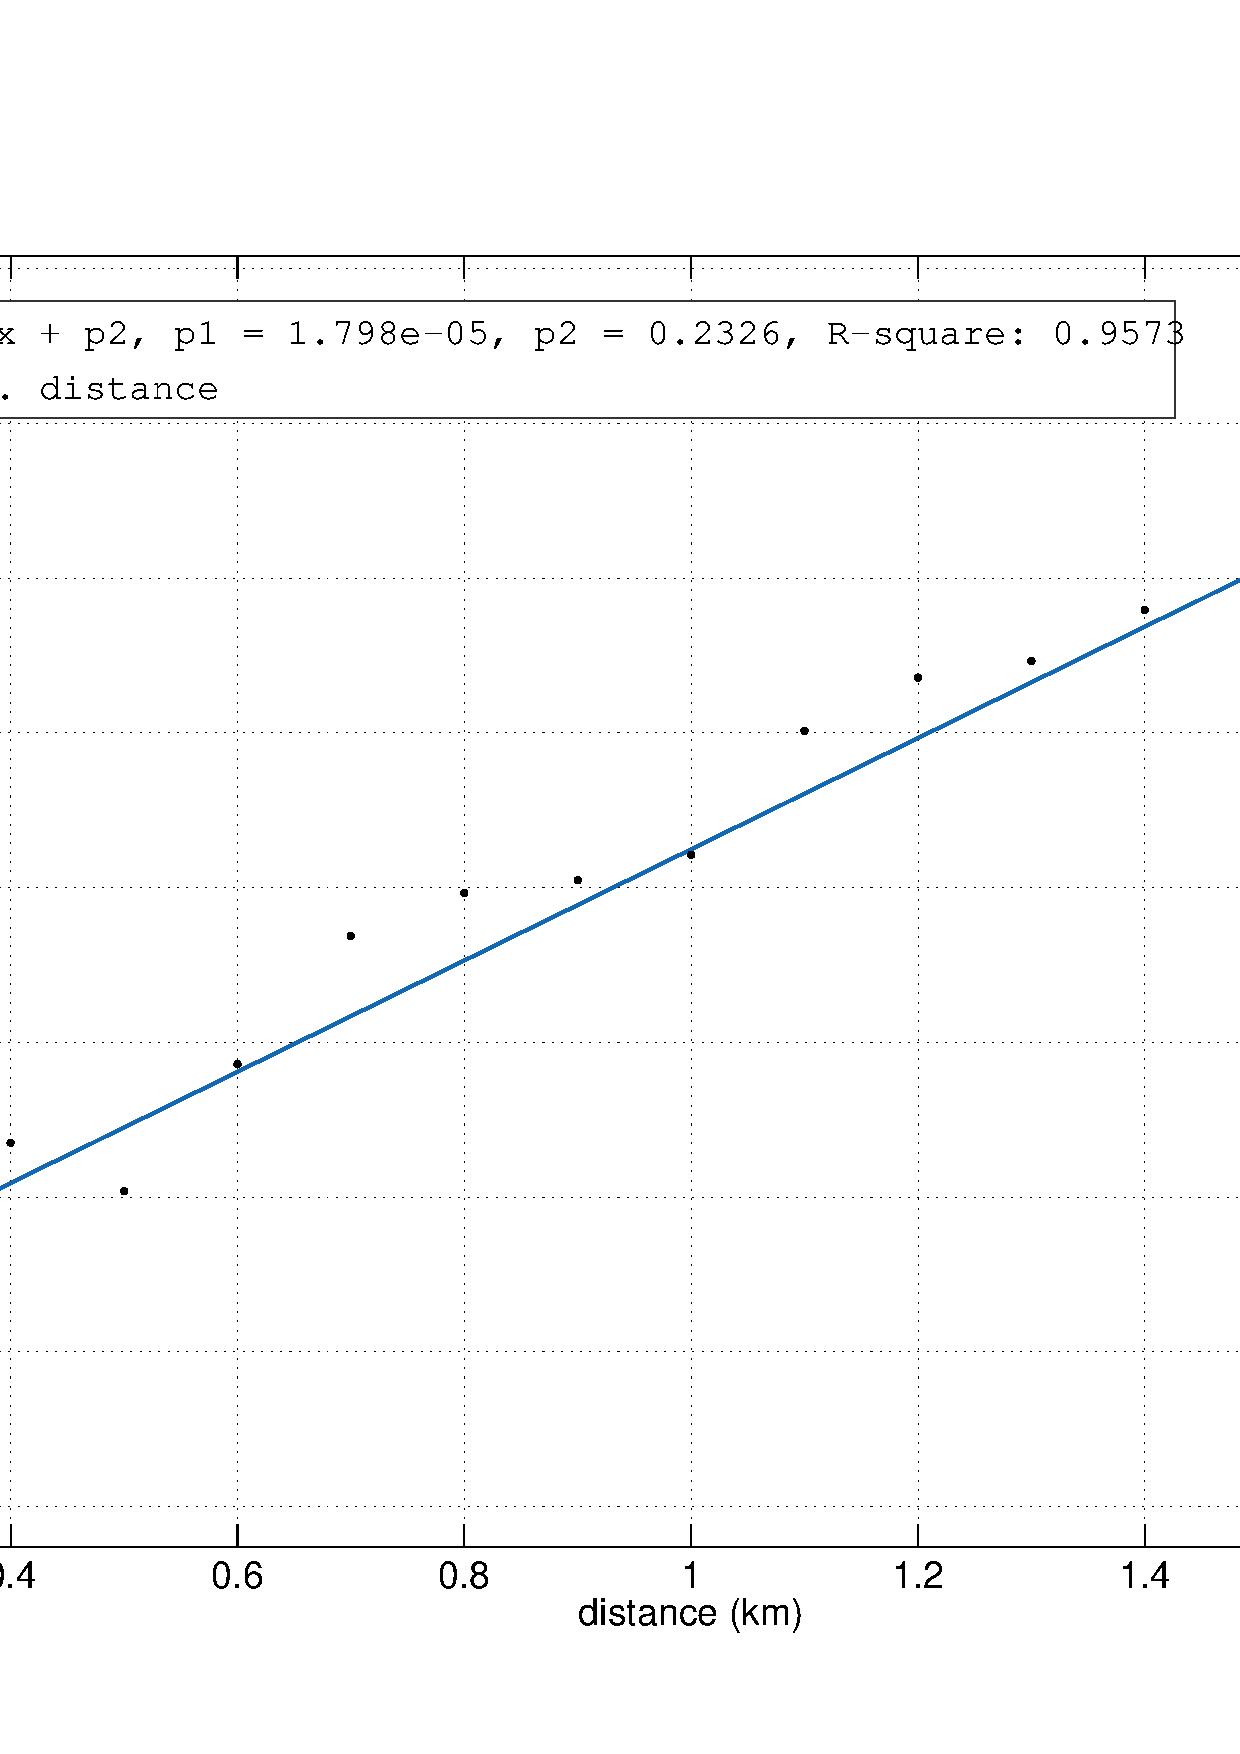
\includegraphics[width=\linewidth]{../figs/fit_curve.pdf}
  \caption{Linear fitting of latency vs. distance}
  \label{fig:fit_curve}
\end{figure}

\subsection{Latency for DC conversation}
\label{sec:latency-dc-conv-1}

\begin{figure}
  \centering
  \includegraphics[width=\linewidth]{../figs/data_center.pdf}
  \caption{The latency measured in DC conversation experiments}
  \label{fig:data_center}
\end{figure}

\subsection{Latency within the Cellular Networks}
\label{sec:latency-with-cell}

\begin{figure}
  \centering
  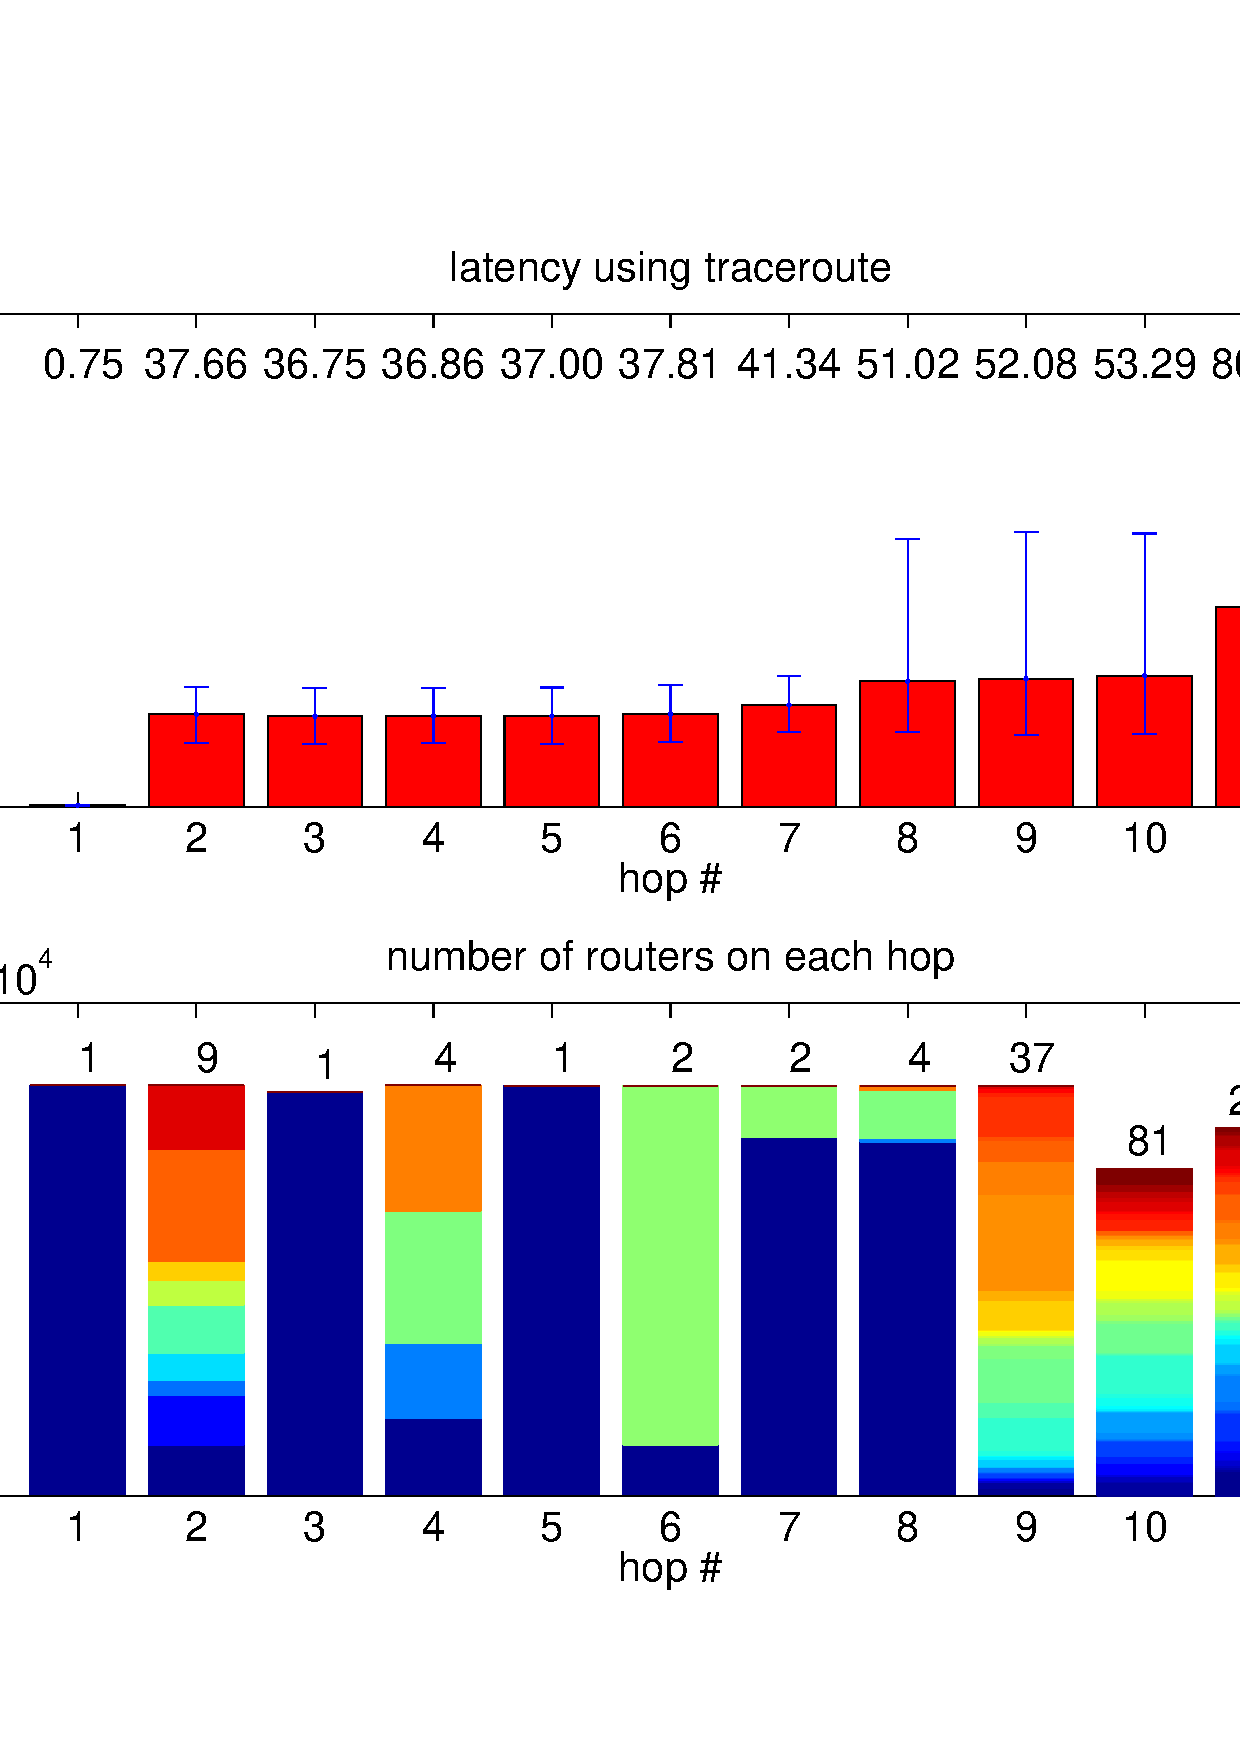
\includegraphics[width=\linewidth]{../figs/mobile_latency.pdf}
  \caption{Latency measured in each hop of AT\&T cellular networks}
  \label{fig:mobile_latency}
\end{figure}

\begin{figure}
  \centering
  \includegraphics[width=\linewidth]{../figs/routing_flaps.pdf}
  \caption{Routing flaps within AT\&T cellular networks}
  \label{fig:mobile_flaps}
\end{figure}

\begin{figure}
  \centering
  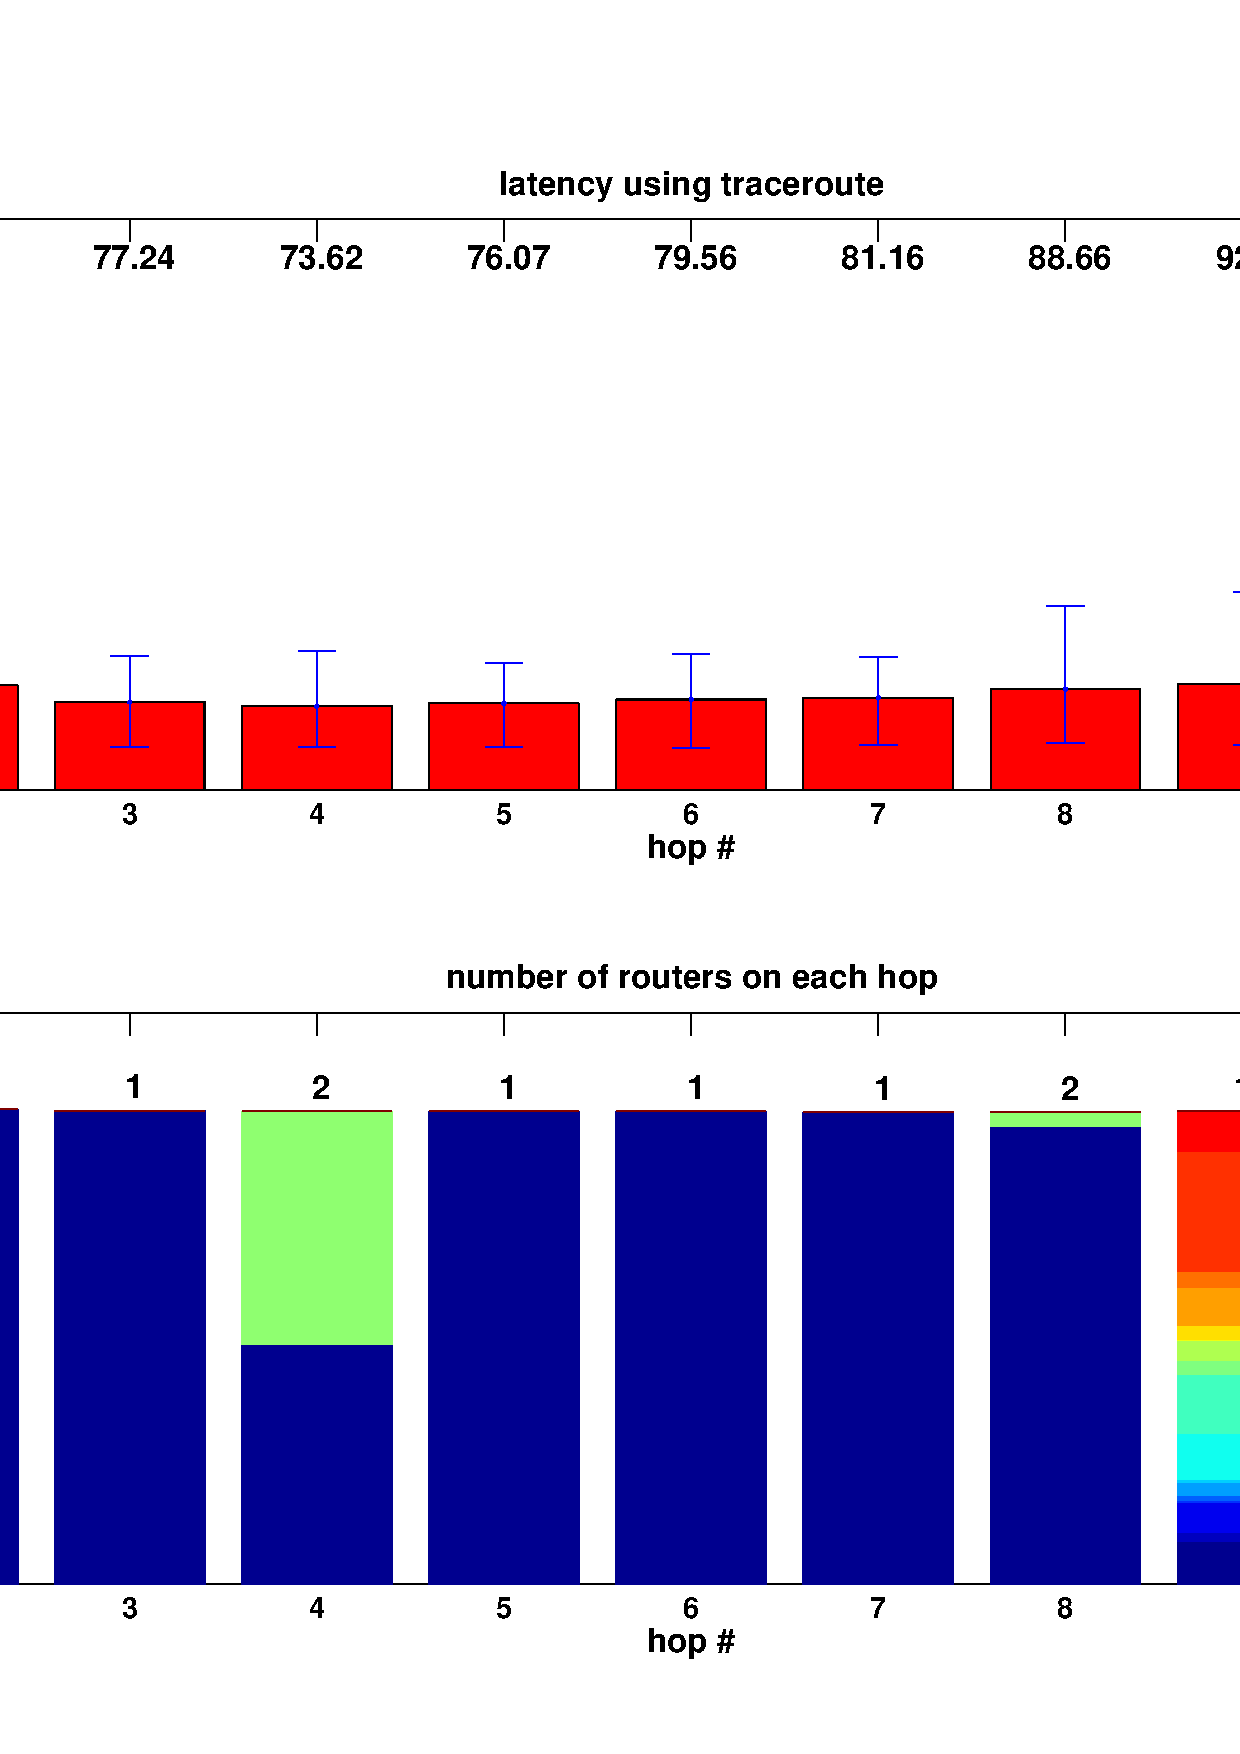
\includegraphics[width=\linewidth]{../figs/mobile_sfo.pdf}
  \caption{Latency when mobile phone is moving between Berkeley and San Francisco}
  \label{fig:mobile_mobile}
\end{figure}

%%% Local Variables: 
%%% mode: latex
%%% TeX-master: "main"
%%% End: 
